\documentclass[twoside]{book}

% Packages required by doxygen
\usepackage{fixltx2e}
\usepackage{calc}
\usepackage{doxygen}
\usepackage{graphicx}
\usepackage[utf8]{inputenc}
\usepackage{makeidx}
\usepackage{multicol}
\usepackage{multirow}
\PassOptionsToPackage{warn}{textcomp}
\usepackage{textcomp}
\usepackage[nointegrals]{wasysym}
\usepackage[table]{xcolor}

% NLS support packages
\usepackage[french]{babel}

% Font selection
\usepackage[T1]{fontenc}
\usepackage{mathptmx}
\usepackage[scaled=.90]{helvet}
\usepackage{courier}
\usepackage{amssymb}
\usepackage{sectsty}
\renewcommand{\familydefault}{\sfdefault}
\allsectionsfont{%
  \fontseries{bc}\selectfont%
  \color{darkgray}%
}
\renewcommand{\DoxyLabelFont}{%
  \fontseries{bc}\selectfont%
  \color{darkgray}%
}
\newcommand{\+}{\discretionary{\mbox{\scriptsize$\hookleftarrow$}}{}{}}

% Page & text layout
\usepackage{geometry}
\geometry{%
  a4paper,%
  top=2.5cm,%
  bottom=2.5cm,%
  left=2.5cm,%
  right=2.5cm%
}
\tolerance=750
\hfuzz=15pt
\hbadness=750
\setlength{\emergencystretch}{15pt}
\setlength{\parindent}{0cm}
\setlength{\parskip}{0.2cm}
\makeatletter
\renewcommand{\paragraph}{%
  \@startsection{paragraph}{4}{0ex}{-1.0ex}{1.0ex}{%
    \normalfont\normalsize\bfseries\SS@parafont%
  }%
}
\renewcommand{\subparagraph}{%
  \@startsection{subparagraph}{5}{0ex}{-1.0ex}{1.0ex}{%
    \normalfont\normalsize\bfseries\SS@subparafont%
  }%
}
\makeatother

% Headers & footers
\usepackage{fancyhdr}
\pagestyle{fancyplain}
\fancyhead[LE]{\fancyplain{}{\bfseries\thepage}}
\fancyhead[CE]{\fancyplain{}{}}
\fancyhead[RE]{\fancyplain{}{\bfseries\leftmark}}
\fancyhead[LO]{\fancyplain{}{\bfseries\rightmark}}
\fancyhead[CO]{\fancyplain{}{}}
\fancyhead[RO]{\fancyplain{}{\bfseries\thepage}}
\fancyfoot[LE]{\fancyplain{}{}}
\fancyfoot[CE]{\fancyplain{}{}}
\fancyfoot[RE]{\fancyplain{}{\bfseries\scriptsize Généré le Mercredi 11 Février 2015 11\+:46\+:25 pour Tic\+\_\+\+Tac\+\_\+\+Toe par Doxygen }}
\fancyfoot[LO]{\fancyplain{}{\bfseries\scriptsize Généré le Mercredi 11 Février 2015 11\+:46\+:25 pour Tic\+\_\+\+Tac\+\_\+\+Toe par Doxygen }}
\fancyfoot[CO]{\fancyplain{}{}}
\fancyfoot[RO]{\fancyplain{}{}}
\renewcommand{\footrulewidth}{0.4pt}
\renewcommand{\chaptermark}[1]{%
  \markboth{#1}{}%
}
\renewcommand{\sectionmark}[1]{%
  \markright{\thesection\ #1}%
}

% Indices & bibliography
\usepackage{natbib}
\usepackage[titles]{tocloft}
\setcounter{tocdepth}{3}
\setcounter{secnumdepth}{5}
\makeindex

% Hyperlinks (required, but should be loaded last)
\usepackage{ifpdf}
\ifpdf
  \usepackage[pdftex,pagebackref=true]{hyperref}
\else
  \usepackage[ps2pdf,pagebackref=true]{hyperref}
\fi
\hypersetup{%
  colorlinks=true,%
  linkcolor=blue,%
  citecolor=blue,%
  unicode%
}

% Custom commands
\newcommand{\clearemptydoublepage}{%
  \newpage{\pagestyle{empty}\cleardoublepage}%
}


%===== C O N T E N T S =====

\begin{document}

% Titlepage & ToC
\hypersetup{pageanchor=false,
             bookmarks=true,
             bookmarksnumbered=true,
             pdfencoding=unicode
            }
\pagenumbering{roman}
\begin{titlepage}
\vspace*{7cm}
\begin{center}%
{\Large Tic\+\_\+\+Tac\+\_\+\+Toe }\\
\vspace*{1cm}
{\large Généré par Doxygen 1.8.8}\\
\vspace*{0.5cm}
{\small Mercredi 11 Février 2015 11:46:25}\\
\end{center}
\end{titlepage}
\clearemptydoublepage
\tableofcontents
\clearemptydoublepage
\pagenumbering{arabic}
\hypersetup{pageanchor=true}

%--- Begin generated contents ---
\chapter{Tic\+\_\+\+Tac\+\_\+\+Toe}
\label{md_README}
\hypertarget{md_README}{}
Famous game of tic tac toe 
\chapter{Index des fichiers}
\section{Liste des fichiers}
Liste de tous les fichiers documentés avec une brève description \+:\begin{DoxyCompactList}
\item\contentsline{section}{\hyperlink{bilbilotheque_8c}{bilbilotheque.\+c} \\*Page contenant les definitons des fonctions importantes a tous les programmes }{\pageref{bilbilotheque_8c}}{}
\item\contentsline{section}{\hyperlink{engine_8c}{engine.\+c} \\*Page contenant toutes les fonctions necessaires au jeu }{\pageref{engine_8c}}{}
\item\contentsline{section}{\hyperlink{header_8h}{header.\+h} \\*Page contenant les defintions de tout ce qui est nécéssaire au tic tac toe }{\pageref{header_8h}}{}
\item\contentsline{section}{\hyperlink{main_8c}{main.\+c} \\*Page contenant le code d'execution du tic tac toe }{\pageref{main_8c}}{}
\end{DoxyCompactList}

\chapter{Documentation des fichiers}
\hypertarget{bilbilotheque_8c}{\section{Référence du fichier bilbilotheque.\+c}
\label{bilbilotheque_8c}\index{bilbilotheque.\+c@{bilbilotheque.\+c}}
}


Page contenant les definitons des fonctions importantes a tous les programmes.  


{\ttfamily \#include \char`\"{}header.\+h\char`\"{}}\\*
Graphe des dépendances par inclusion de bilbilotheque.\+c\+:\nopagebreak
\begin{figure}[H]
\begin{center}
\leavevmode
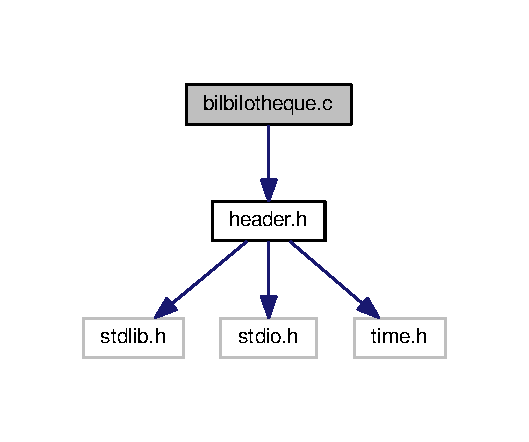
\includegraphics[width=254pt]{bilbilotheque_8c__incl}
\end{center}
\end{figure}
\subsection*{Fonctions}
\begin{DoxyCompactItemize}
\item 
\hypertarget{bilbilotheque_8c_aaeeedbd134251291fe79c71c943ec899}{void \hyperlink{bilbilotheque_8c_aaeeedbd134251291fe79c71c943ec899}{aleatoire} (void)}\label{bilbilotheque_8c_aaeeedbd134251291fe79c71c943ec899}

\begin{DoxyCompactList}\small\item\em Fonction permettant de creer l'aleatoire. \end{DoxyCompactList}\item 
int \hyperlink{bilbilotheque_8c_a5d77334ef0eb544c90e47f78b6e898cd}{verif\+\_\+saisie} (int petit, int grand)
\begin{DoxyCompactList}\small\item\em Fonction permettant de verifier si la saisie de l'utilisateur est correcte. \end{DoxyCompactList}\item 
void \hyperlink{bilbilotheque_8c_afdabedbdaec06f1a4ab234044b4df6fc}{affiche\+\_\+entrer} (int tmp)
\begin{DoxyCompactList}\small\item\em Fonction permettant l'affichage d'un certain nombre de ligne vide. \end{DoxyCompactList}\end{DoxyCompactItemize}


\subsection{Description détaillée}
Page contenant les definitons des fonctions importantes a tous les programmes. 

\begin{DoxyAuthor}{Auteur}
triodebeignets 
\end{DoxyAuthor}
\begin{DoxyVersion}{Version}
1.\+0 
\end{DoxyVersion}
\begin{DoxyDate}{Date}
22 Janvier 2014 
\end{DoxyDate}


\subsection{Documentation des fonctions}
\hypertarget{bilbilotheque_8c_afdabedbdaec06f1a4ab234044b4df6fc}{\index{bilbilotheque.\+c@{bilbilotheque.\+c}!affiche\+\_\+entrer@{affiche\+\_\+entrer}}
\index{affiche\+\_\+entrer@{affiche\+\_\+entrer}!bilbilotheque.\+c@{bilbilotheque.\+c}}
\subsubsection[{affiche\+\_\+entrer}]{\setlength{\rightskip}{0pt plus 5cm}void affiche\+\_\+entrer (
\begin{DoxyParamCaption}
\item[{int}]{tmp}
\end{DoxyParamCaption}
)}}\label{bilbilotheque_8c_afdabedbdaec06f1a4ab234044b4df6fc}


Fonction permettant l'affichage d'un certain nombre de ligne vide. 


\begin{DoxyParams}{Paramètres}
{\em int} & tmp nombre de retour chariot à afficher \\
\hline
\end{DoxyParams}
\hypertarget{bilbilotheque_8c_a5d77334ef0eb544c90e47f78b6e898cd}{\index{bilbilotheque.\+c@{bilbilotheque.\+c}!verif\+\_\+saisie@{verif\+\_\+saisie}}
\index{verif\+\_\+saisie@{verif\+\_\+saisie}!bilbilotheque.\+c@{bilbilotheque.\+c}}
\subsubsection[{verif\+\_\+saisie}]{\setlength{\rightskip}{0pt plus 5cm}int verif\+\_\+saisie (
\begin{DoxyParamCaption}
\item[{int}]{petit, }
\item[{int}]{grand}
\end{DoxyParamCaption}
)}}\label{bilbilotheque_8c_a5d77334ef0eb544c90e47f78b6e898cd}


Fonction permettant de verifier si la saisie de l'utilisateur est correcte. 


\begin{DoxyParams}{Paramètres}
{\em int} & petit, int grand paramètre pour verifier si le nombre entrer n'est pas trop grand ou trop petit \\
\hline
\end{DoxyParams}
\begin{DoxyReturn}{Renvoie}
renvoi le nombre entrer par l'utilisateur 
\end{DoxyReturn}

\hypertarget{engine_8c}{\section{Référence du fichier engine.\+c}
\label{engine_8c}\index{engine.\+c@{engine.\+c}}
}


Page contenant toutes les fonctions necessaires au jeu.  


{\ttfamily \#include \char`\"{}header.\+h\char`\"{}}\\*
Graphe des dépendances par inclusion de engine.\+c\+:
\nopagebreak
\begin{figure}[H]
\begin{center}
\leavevmode
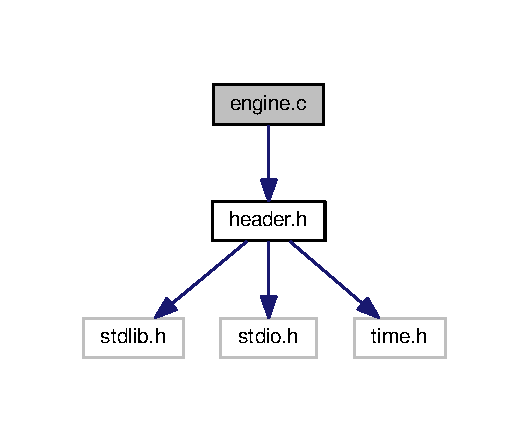
\includegraphics[width=254pt]{engine_8c__incl}
\end{center}
\end{figure}
\subsection*{Fonctions}
\begin{DoxyCompactItemize}
\item 
\hypertarget{engine_8c_aa268c4c4b7f046ee706f57246ef1573a}{\hyperlink{header_8h_ac77a18127be97d5680b10233bf102d09}{t\+\_\+joueur} \hyperlink{engine_8c_aa268c4c4b7f046ee706f57246ef1573a}{choix\+\_\+joueur} (void)}\label{engine_8c_aa268c4c4b7f046ee706f57246ef1573a}

\begin{DoxyCompactList}\small\item\em Fonction permettant de savoir quel joueur doit jouer. \end{DoxyCompactList}\item 
\hypertarget{engine_8c_a3e120efb274a01b45af7bb3616effc8c}{\hyperlink{header_8h_ac77a18127be97d5680b10233bf102d09}{t\+\_\+joueur} \hyperlink{engine_8c_a3e120efb274a01b45af7bb3616effc8c}{premier\+\_\+joueur} (void)}\label{engine_8c_a3e120efb274a01b45af7bb3616effc8c}

\begin{DoxyCompactList}\small\item\em Fonction permettant de savoir qui du joueur 1 ou du joueur 2 va commencer a jouer. \end{DoxyCompactList}\item 
\hypertarget{engine_8c_ac56a10e278cb046501b86d931c3600b8}{void \hyperlink{engine_8c_ac56a10e278cb046501b86d931c3600b8}{victoire} (void)}\label{engine_8c_ac56a10e278cb046501b86d931c3600b8}

\begin{DoxyCompactList}\small\item\em Fonction permettant d'afficher le joueur gagnant. \end{DoxyCompactList}\item 
\hypertarget{engine_8c_a18729c7b80c8918f251c94dfd1dab17b}{int \hyperlink{engine_8c_a18729c7b80c8918f251c94dfd1dab17b}{fin\+\_\+jeu} (void)}\label{engine_8c_a18729c7b80c8918f251c94dfd1dab17b}

\begin{DoxyCompactList}\small\item\em Fonction permettant de verifier si la partie est finie. \end{DoxyCompactList}\item 
\hypertarget{engine_8c_ad78f824108b1b985e899d092e810392f}{int \hyperlink{engine_8c_ad78f824108b1b985e899d092e810392f}{verif\+\_\+colonnes} (void)}\label{engine_8c_ad78f824108b1b985e899d092e810392f}

\begin{DoxyCompactList}\small\item\em Fonction permettant de verifier si une colonne de la table de jeu est rempli de m�me pions. \end{DoxyCompactList}\item 
\hypertarget{engine_8c_ab2da4309c4408450c59af322b4707f51}{int \hyperlink{engine_8c_ab2da4309c4408450c59af322b4707f51}{verif\+\_\+lignes} (void)}\label{engine_8c_ab2da4309c4408450c59af322b4707f51}

\begin{DoxyCompactList}\small\item\em Fonction permettant de verifier si une colonne de la table de jeu est rempli de m�me pions. \end{DoxyCompactList}\item 
\hypertarget{engine_8c_a02d8aac1c040e305611ffe0ede6de0e3}{int \hyperlink{engine_8c_a02d8aac1c040e305611ffe0ede6de0e3}{verif\+\_\+diagonales} (void)}\label{engine_8c_a02d8aac1c040e305611ffe0ede6de0e3}

\begin{DoxyCompactList}\small\item\em Fonction permettant de verifier si une colonne de la table de jeu est rempli de m�me pions. \end{DoxyCompactList}\item 
void \hyperlink{engine_8c_afdfd7971780376a3fd4ce80ca40805b5}{remplir\+\_\+table} (\hyperlink{header_8h_ac77a18127be97d5680b10233bf102d09}{t\+\_\+joueur} joueur)
\begin{DoxyCompactList}\small\item\em Fonction permettant de remplir une case de la table par le joueur. \end{DoxyCompactList}\item 
\hypertarget{engine_8c_a568a55cbffe29dee8b6f668065977d61}{void \hyperlink{engine_8c_a568a55cbffe29dee8b6f668065977d61}{init\+\_\+table} (void)}\label{engine_8c_a568a55cbffe29dee8b6f668065977d61}

\begin{DoxyCompactList}\small\item\em Fonction permettant de passer a l'etat vide la matrice du jeu. \end{DoxyCompactList}\item 
\hypertarget{engine_8c_a4632d20b554a49a93a9f12ef0e480f95}{void \hyperlink{engine_8c_a4632d20b554a49a93a9f12ef0e480f95}{affichage\+\_\+table} (void)}\label{engine_8c_a4632d20b554a49a93a9f12ef0e480f95}

\begin{DoxyCompactList}\small\item\em Fonction permettant d'afficher la table de jeu. \end{DoxyCompactList}\item 
\hypertarget{engine_8c_a37a665341a6c6d1c93c28842798a450e}{void \hyperlink{engine_8c_a37a665341a6c6d1c93c28842798a450e}{affiche\+\_\+tour} (\hyperlink{header_8h_ac77a18127be97d5680b10233bf102d09}{t\+\_\+joueur} joueur)}\label{engine_8c_a37a665341a6c6d1c93c28842798a450e}

\begin{DoxyCompactList}\small\item\em Fonction permettant d'afficher quel joueur va jouer. \end{DoxyCompactList}\end{DoxyCompactItemize}


\subsection{Description détaillée}
Page contenant toutes les fonctions necessaires au jeu. 

\begin{DoxyAuthor}{Auteur}
triodebeignets 
\end{DoxyAuthor}
\begin{DoxyVersion}{Version}
1.\+0 
\end{DoxyVersion}
\begin{DoxyDate}{Date}
19 Janvier 2014 
\end{DoxyDate}


\subsection{Documentation des fonctions}
\hypertarget{engine_8c_afdfd7971780376a3fd4ce80ca40805b5}{\index{engine.\+c@{engine.\+c}!remplir\+\_\+table@{remplir\+\_\+table}}
\index{remplir\+\_\+table@{remplir\+\_\+table}!engine.\+c@{engine.\+c}}
\subsubsection[{remplir\+\_\+table}]{\setlength{\rightskip}{0pt plus 5cm}void remplir\+\_\+table (
\begin{DoxyParamCaption}
\item[{{\bf t\+\_\+joueur}}]{joueur}
\end{DoxyParamCaption}
)}}\label{engine_8c_afdfd7971780376a3fd4ce80ca40805b5}


Fonction permettant de remplir une case de la table par le joueur. 


\begin{DoxyParams}{Paramètres}
{\em t\+\_\+joueur} & joueur permet de savoir quel joueur jouer \\
\hline
\end{DoxyParams}

\hypertarget{header_8h}{\section{Référence du fichier header.\+h}
\label{header_8h}\index{header.\+h@{header.\+h}}
}


Page contenant les defintions de tout ce qui est nécéssaire au tic tac toe.  


{\ttfamily \#include $<$stdlib.\+h$>$}\\*
{\ttfamily \#include $<$stdio.\+h$>$}\\*
{\ttfamily \#include $<$time.\+h$>$}\\*
Graphe des dépendances par inclusion de header.\+h\+:\nopagebreak
\begin{figure}[H]
\begin{center}
\leavevmode
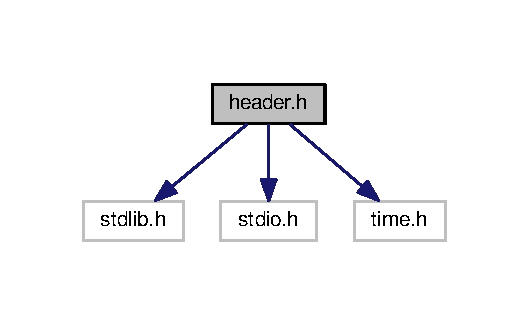
\includegraphics[width=254pt]{header_8h__incl}
\end{center}
\end{figure}
Ce graphe montre quels fichiers incluent directement ou indirectement ce fichier \+:
\nopagebreak
\begin{figure}[H]
\begin{center}
\leavevmode
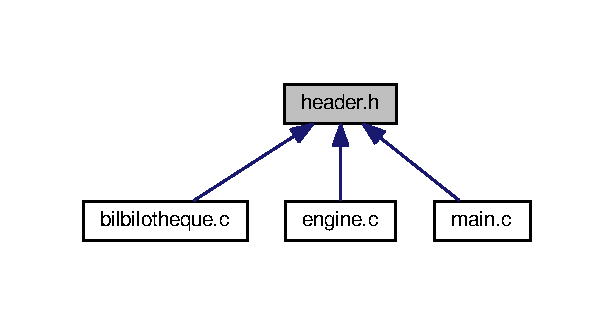
\includegraphics[width=294pt]{header_8h__dep__incl}
\end{center}
\end{figure}
\subsection*{Macros}
\begin{DoxyCompactItemize}
\item 
\hypertarget{header_8h_a0240ac851181b84ac374872dc5434ee4}{\#define {\bfseries N}~3}\label{header_8h_a0240ac851181b84ac374872dc5434ee4}

\end{DoxyCompactItemize}
\subsection*{Énumérations}
\begin{DoxyCompactItemize}
\item 
\hypertarget{header_8h_ab21a60e1517c8d253cc83c12f6e027f3}{enum \hyperlink{header_8h_ab21a60e1517c8d253cc83c12f6e027f3}{t\+\_\+case} \{ {\bfseries vide}, 
{\bfseries croix}, 
{\bfseries rond}
 \}}\label{header_8h_ab21a60e1517c8d253cc83c12f6e027f3}

\begin{DoxyCompactList}\small\item\em definition d'une énumération de type t\+\_\+case representant le contenu des cases de la table de jeu (rond pour joueur 2 et croix pour joueur 1) \end{DoxyCompactList}\item 
\hypertarget{header_8h_ac77a18127be97d5680b10233bf102d09}{enum \hyperlink{header_8h_ac77a18127be97d5680b10233bf102d09}{t\+\_\+joueur} \{ {\bfseries joueur1}, 
{\bfseries joueur2}
 \}}\label{header_8h_ac77a18127be97d5680b10233bf102d09}

\begin{DoxyCompactList}\small\item\em definition d'une énumération de type t\+\_\+joueur permettant de connaitre le joueur en cours de jeu \end{DoxyCompactList}\end{DoxyCompactItemize}
\subsection*{Fonctions}
\begin{DoxyCompactItemize}
\item 
\hypertarget{header_8h_aaeeedbd134251291fe79c71c943ec899}{void \hyperlink{header_8h_aaeeedbd134251291fe79c71c943ec899}{aleatoire} (void)}\label{header_8h_aaeeedbd134251291fe79c71c943ec899}

\begin{DoxyCompactList}\small\item\em Fonction permettant de creer l'aleatoire. \end{DoxyCompactList}\item 
int \hyperlink{header_8h_a5d77334ef0eb544c90e47f78b6e898cd}{verif\+\_\+saisie} (int petit, int grand)
\begin{DoxyCompactList}\small\item\em Fonction permettant de verifier si la saisie de l'utilisateur est correcte. \end{DoxyCompactList}\item 
void \hyperlink{header_8h_afdabedbdaec06f1a4ab234044b4df6fc}{affiche\+\_\+entrer} (int tmp)
\begin{DoxyCompactList}\small\item\em Fonction permettant l'affichage d'un certain nombre de ligne vide. \end{DoxyCompactList}\item 
\hypertarget{header_8h_aa268c4c4b7f046ee706f57246ef1573a}{\hyperlink{header_8h_ac77a18127be97d5680b10233bf102d09}{t\+\_\+joueur} \hyperlink{header_8h_aa268c4c4b7f046ee706f57246ef1573a}{choix\+\_\+joueur} (void)}\label{header_8h_aa268c4c4b7f046ee706f57246ef1573a}

\begin{DoxyCompactList}\small\item\em Fonction permettant de savoir quel joueur doit jouer. \end{DoxyCompactList}\item 
\hypertarget{header_8h_a3e120efb274a01b45af7bb3616effc8c}{\hyperlink{header_8h_ac77a18127be97d5680b10233bf102d09}{t\+\_\+joueur} \hyperlink{header_8h_a3e120efb274a01b45af7bb3616effc8c}{premier\+\_\+joueur} (void)}\label{header_8h_a3e120efb274a01b45af7bb3616effc8c}

\begin{DoxyCompactList}\small\item\em Fonction permettant de savoir qui du joueur 1 ou du joueur 2 va commencer a jouer. \end{DoxyCompactList}\item 
\hypertarget{header_8h_ac56a10e278cb046501b86d931c3600b8}{void \hyperlink{header_8h_ac56a10e278cb046501b86d931c3600b8}{victoire} (void)}\label{header_8h_ac56a10e278cb046501b86d931c3600b8}

\begin{DoxyCompactList}\small\item\em Fonction permettant d'afficher le joueur gagnant. \end{DoxyCompactList}\item 
\hypertarget{header_8h_a18729c7b80c8918f251c94dfd1dab17b}{int \hyperlink{header_8h_a18729c7b80c8918f251c94dfd1dab17b}{fin\+\_\+jeu} (void)}\label{header_8h_a18729c7b80c8918f251c94dfd1dab17b}

\begin{DoxyCompactList}\small\item\em Fonction permettant de verifier si la partie est finie. \end{DoxyCompactList}\item 
\hypertarget{header_8h_ad78f824108b1b985e899d092e810392f}{int \hyperlink{header_8h_ad78f824108b1b985e899d092e810392f}{verif\+\_\+colonnes} (void)}\label{header_8h_ad78f824108b1b985e899d092e810392f}

\begin{DoxyCompactList}\small\item\em Fonction permettant de verifier si une colonne de la table de jeu est rempli de m�me pions. \end{DoxyCompactList}\item 
\hypertarget{header_8h_ab2da4309c4408450c59af322b4707f51}{int \hyperlink{header_8h_ab2da4309c4408450c59af322b4707f51}{verif\+\_\+lignes} (void)}\label{header_8h_ab2da4309c4408450c59af322b4707f51}

\begin{DoxyCompactList}\small\item\em Fonction permettant de verifier si une colonne de la table de jeu est rempli de m�me pions. \end{DoxyCompactList}\item 
\hypertarget{header_8h_a02d8aac1c040e305611ffe0ede6de0e3}{int \hyperlink{header_8h_a02d8aac1c040e305611ffe0ede6de0e3}{verif\+\_\+diagonales} (void)}\label{header_8h_a02d8aac1c040e305611ffe0ede6de0e3}

\begin{DoxyCompactList}\small\item\em Fonction permettant de verifier si une colonne de la table de jeu est rempli de m�me pions. \end{DoxyCompactList}\item 
void \hyperlink{header_8h_afdfd7971780376a3fd4ce80ca40805b5}{remplir\+\_\+table} (\hyperlink{header_8h_ac77a18127be97d5680b10233bf102d09}{t\+\_\+joueur} joueur)
\begin{DoxyCompactList}\small\item\em Fonction permettant de remplir une case de la table par le joueur. \end{DoxyCompactList}\item 
\hypertarget{header_8h_a568a55cbffe29dee8b6f668065977d61}{void \hyperlink{header_8h_a568a55cbffe29dee8b6f668065977d61}{init\+\_\+table} (void)}\label{header_8h_a568a55cbffe29dee8b6f668065977d61}

\begin{DoxyCompactList}\small\item\em Fonction permettant de passer a l'etat vide la matrice du jeu. \end{DoxyCompactList}\item 
\hypertarget{header_8h_a3e6705b70658a81654386ae9bc467ec8}{void \hyperlink{header_8h_a3e6705b70658a81654386ae9bc467ec8}{affichage\+\_\+table} (void)}\label{header_8h_a3e6705b70658a81654386ae9bc467ec8}

\begin{DoxyCompactList}\small\item\em Fonction permettant d'afficher la table de jeu. \end{DoxyCompactList}\item 
\hypertarget{header_8h_a37a665341a6c6d1c93c28842798a450e}{void \hyperlink{header_8h_a37a665341a6c6d1c93c28842798a450e}{affiche\+\_\+tour} (\hyperlink{header_8h_ac77a18127be97d5680b10233bf102d09}{t\+\_\+joueur} joueur)}\label{header_8h_a37a665341a6c6d1c93c28842798a450e}

\begin{DoxyCompactList}\small\item\em Fonction permettant d'afficher quel joueur va jouer. \end{DoxyCompactList}\end{DoxyCompactItemize}
\subsection*{Variables}
\begin{DoxyCompactItemize}
\item 
\hypertarget{header_8h_a25df6dc581cce931468011cdb1c5741d}{\hyperlink{header_8h_ab21a60e1517c8d253cc83c12f6e027f3}{t\+\_\+case} {\bfseries table} \mbox{[}N\mbox{]}\mbox{[}N\mbox{]}}\label{header_8h_a25df6dc581cce931468011cdb1c5741d}

\item 
\hypertarget{header_8h_ab62d6cef413f5ca703848194be177ec1}{int {\bfseries nb\+\_\+tour}}\label{header_8h_ab62d6cef413f5ca703848194be177ec1}

\end{DoxyCompactItemize}


\subsection{Description détaillée}
Page contenant les defintions de tout ce qui est nécéssaire au tic tac toe. 

\begin{DoxyAuthor}{Auteur}
triodebeignets 
\end{DoxyAuthor}
\begin{DoxyVersion}{Version}
1.\+0 
\end{DoxyVersion}
\begin{DoxyDate}{Date}
19 Janvier 2014 
\end{DoxyDate}


\subsection{Documentation des fonctions}
\hypertarget{header_8h_afdabedbdaec06f1a4ab234044b4df6fc}{\index{header.\+h@{header.\+h}!affiche\+\_\+entrer@{affiche\+\_\+entrer}}
\index{affiche\+\_\+entrer@{affiche\+\_\+entrer}!header.\+h@{header.\+h}}
\subsubsection[{affiche\+\_\+entrer}]{\setlength{\rightskip}{0pt plus 5cm}void affiche\+\_\+entrer (
\begin{DoxyParamCaption}
\item[{int}]{tmp}
\end{DoxyParamCaption}
)}}\label{header_8h_afdabedbdaec06f1a4ab234044b4df6fc}


Fonction permettant l'affichage d'un certain nombre de ligne vide. 


\begin{DoxyParams}{Paramètres}
{\em int} & tmp nombre de retour chariot à afficher \\
\hline
\end{DoxyParams}
\hypertarget{header_8h_afdfd7971780376a3fd4ce80ca40805b5}{\index{header.\+h@{header.\+h}!remplir\+\_\+table@{remplir\+\_\+table}}
\index{remplir\+\_\+table@{remplir\+\_\+table}!header.\+h@{header.\+h}}
\subsubsection[{remplir\+\_\+table}]{\setlength{\rightskip}{0pt plus 5cm}void remplir\+\_\+table (
\begin{DoxyParamCaption}
\item[{{\bf t\+\_\+joueur}}]{joueur}
\end{DoxyParamCaption}
)}}\label{header_8h_afdfd7971780376a3fd4ce80ca40805b5}


Fonction permettant de remplir une case de la table par le joueur. 


\begin{DoxyParams}{Paramètres}
{\em t\+\_\+joueur} & joueur permet de savoir quel joueur jouer \\
\hline
\end{DoxyParams}
\hypertarget{header_8h_a5d77334ef0eb544c90e47f78b6e898cd}{\index{header.\+h@{header.\+h}!verif\+\_\+saisie@{verif\+\_\+saisie}}
\index{verif\+\_\+saisie@{verif\+\_\+saisie}!header.\+h@{header.\+h}}
\subsubsection[{verif\+\_\+saisie}]{\setlength{\rightskip}{0pt plus 5cm}int verif\+\_\+saisie (
\begin{DoxyParamCaption}
\item[{int}]{petit, }
\item[{int}]{grand}
\end{DoxyParamCaption}
)}}\label{header_8h_a5d77334ef0eb544c90e47f78b6e898cd}


Fonction permettant de verifier si la saisie de l'utilisateur est correcte. 


\begin{DoxyParams}{Paramètres}
{\em int} & petit, int grand paramètre pour verifier si le nombre entrer n'est pas trop grand ou trop petit \\
\hline
\end{DoxyParams}
\begin{DoxyReturn}{Renvoie}
renvoi le nombre entrer par l'utilisateur 
\end{DoxyReturn}

\hypertarget{main_8c}{\section{Référence du fichier main.\+c}
\label{main_8c}\index{main.\+c@{main.\+c}}
}


Page contenant le code d'execution du tic tac toe.  


{\ttfamily \#include \char`\"{}header.\+h\char`\"{}}\\*
Graphe des dépendances par inclusion de main.\+c\+:\nopagebreak
\begin{figure}[H]
\begin{center}
\leavevmode
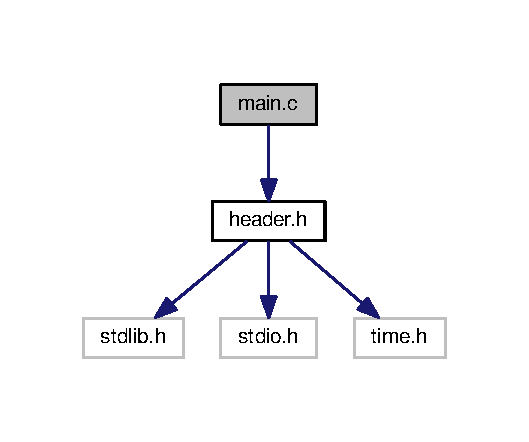
\includegraphics[width=254pt]{main_8c__incl}
\end{center}
\end{figure}
\subsection*{Fonctions}
\begin{DoxyCompactItemize}
\item 
\hypertarget{main_8c_ae66f6b31b5ad750f1fe042a706a4e3d4}{int {\bfseries main} ()}\label{main_8c_ae66f6b31b5ad750f1fe042a706a4e3d4}

\end{DoxyCompactItemize}
\subsection*{Variables}
\begin{DoxyCompactItemize}
\item 
\hypertarget{main_8c_a25df6dc581cce931468011cdb1c5741d}{\hyperlink{header_8h_ab21a60e1517c8d253cc83c12f6e027f3}{t\+\_\+case} {\bfseries table} \mbox{[}N\mbox{]}\mbox{[}N\mbox{]}}\label{main_8c_a25df6dc581cce931468011cdb1c5741d}

\item 
\hypertarget{main_8c_ab62d6cef413f5ca703848194be177ec1}{int {\bfseries nb\+\_\+tour} = 0}\label{main_8c_ab62d6cef413f5ca703848194be177ec1}

\end{DoxyCompactItemize}


\subsection{Description détaillée}
Page contenant le code d'execution du tic tac toe. 

\begin{DoxyAuthor}{Auteur}
triodebeignets 
\end{DoxyAuthor}
\begin{DoxyVersion}{Version}
1.\+0 
\end{DoxyVersion}
\begin{DoxyDate}{Date}
19 Janvier 2014 
\end{DoxyDate}

%--- End generated contents ---

% Index
\newpage
\phantomsection
\addcontentsline{toc}{chapter}{Index}
\printindex

\end{document}
